% Options for packages loaded elsewhere
\PassOptionsToPackage{unicode}{hyperref}
\PassOptionsToPackage{hyphens}{url}
\PassOptionsToPackage{dvipsnames,svgnames,x11names}{xcolor}
%
\documentclass[
  oneside]{book}
\usepackage{amsmath,amssymb}
\usepackage{lmodern}
\usepackage{iftex}
\ifPDFTeX
  \usepackage[T1]{fontenc}
  \usepackage[utf8]{inputenc}
  \usepackage{textcomp} % provide euro and other symbols
\else % if luatex or xetex
  \usepackage{unicode-math}
  \defaultfontfeatures{Scale=MatchLowercase}
  \defaultfontfeatures[\rmfamily]{Ligatures=TeX,Scale=1}
\fi
% Use upquote if available, for straight quotes in verbatim environments
\IfFileExists{upquote.sty}{\usepackage{upquote}}{}
\IfFileExists{microtype.sty}{% use microtype if available
  \usepackage[]{microtype}
  \UseMicrotypeSet[protrusion]{basicmath} % disable protrusion for tt fonts
}{}
\makeatletter
\@ifundefined{KOMAClassName}{% if non-KOMA class
  \IfFileExists{parskip.sty}{%
    \usepackage{parskip}
  }{% else
    \setlength{\parindent}{0pt}
    \setlength{\parskip}{6pt plus 2pt minus 1pt}}
}{% if KOMA class
  \KOMAoptions{parskip=half}}
\makeatother
\usepackage{xcolor}
\usepackage{longtable,booktabs,array}
\usepackage{calc} % for calculating minipage widths
% Correct order of tables after \paragraph or \subparagraph
\usepackage{etoolbox}
\makeatletter
\patchcmd\longtable{\par}{\if@noskipsec\mbox{}\fi\par}{}{}
\makeatother
% Allow footnotes in longtable head/foot
\IfFileExists{footnotehyper.sty}{\usepackage{footnotehyper}}{\usepackage{footnote}}
\makesavenoteenv{longtable}
\usepackage{graphicx}
\makeatletter
\def\maxwidth{\ifdim\Gin@nat@width>\linewidth\linewidth\else\Gin@nat@width\fi}
\def\maxheight{\ifdim\Gin@nat@height>\textheight\textheight\else\Gin@nat@height\fi}
\makeatother
% Scale images if necessary, so that they will not overflow the page
% margins by default, and it is still possible to overwrite the defaults
% using explicit options in \includegraphics[width, height, ...]{}
\setkeys{Gin}{width=\maxwidth,height=\maxheight,keepaspectratio}
% Set default figure placement to htbp
\makeatletter
\def\fps@figure{htbp}
\makeatother
\setlength{\emergencystretch}{3em} % prevent overfull lines
\providecommand{\tightlist}{%
  \setlength{\itemsep}{0pt}\setlength{\parskip}{0pt}}
\setcounter{secnumdepth}{-\maxdimen} % remove section numbering
\ifLuaTeX
\usepackage[bidi=basic]{babel}
\else
\usepackage[bidi=default]{babel}
\fi
\babelprovide[main,import]{ngerman}
% get rid of language-specific shorthands (see #6817):
\let\LanguageShortHands\languageshorthands
\def\languageshorthands#1{}
\usepackage{booktabs}
\ifLuaTeX
  \usepackage{selnolig}  % disable illegal ligatures
\fi
\usepackage[]{natbib}
\bibliographystyle{plainnat}
\IfFileExists{bookmark.sty}{\usepackage{bookmark}}{\usepackage{hyperref}}
\IfFileExists{xurl.sty}{\usepackage{xurl}}{} % add URL line breaks if available
\urlstyle{same} % disable monospaced font for URLs
\hypersetup{
  pdftitle={Case Study ``Linearmotor''},
  pdfauthor={Martin Schobben},
  pdflang={de},
  colorlinks=true,
  linkcolor={Maroon},
  filecolor={Maroon},
  citecolor={Blue},
  urlcolor={blue},
  pdfcreator={LaTeX via pandoc}}

\title{Case Study ``Linearmotor''}
\author{Martin Schobben}
\date{20 Sep, 2022}

\begin{document}
\maketitle

\hypertarget{section}{%
\section*{}\label{section}}
\addcontentsline{toc}{section}{}

\hypertarget{aktuellen-stand-der-wissenschaft-und-technik}{%
\section{Aktuellen Stand der Wissenschaft und Technik}\label{aktuellen-stand-der-wissenschaft-und-technik}}

Linearmotoren sind am besten bekannt aus ihrer Anwendung in linearen Transportsystemen (wie dem ``Maglev''), die bereits seit einigen Jahrzehnten in Betrieb sind und in mehreren Städten auf der ganzen Welt ihren Dienst tun \citep{hellinger2009, palka2021}. Die Linearmotoren, die diese Transportsysteme antreiben, wurden bereits im 19. und frühen 20. Jahrhundert patentiert und Anwendungen entstanden in den späten 1940er Jahren durch den Visionär Eric Laithwaite vom Imperial College in London \citep{hellinger2009}. Die Anwendung von Linearmotoren für Transportsysteme in der zweiten Hälfte des 20. Jahrhunderts stimulierte eine rasante Entwicklung von Linearmotoren. Dies enthüllte auch die Konstruktionsvorteile des Linearmotors gegenüber herkömmlichen Rotationsmotoren, wie zum Beispiel steuerbare Normalkräfte, direkter Schub ohne Haftung zwischen Rädern und Schienen, wobei letzterer zu geringerem Verschleiß der Kontaktpunkte und damit zu weniger Wartungsaufwand führt. Aufgrund der fortschreitenden Automatisierung vieler Prozesse werden Linearmotoren heutzutage zunehmend in vielen hochpräzisen Industriezweigen eingesetzt, darunter: Öl und Gas, medizinischen Laboren, chirurgische Geräte und Implantate sowie die Herstellung von Halbleiterchips, wodurch sie langsam die traditionellen mechanischen, hydraulischen oder pneumatischen Linearmotoren ersetzen \citep{gieras2018}.

Rotations- und Linearmotoren sind ähnlich aufgebaut, aber anstelle eines Rotors, der sich in einem zylindrischen Mantel aus Blech (Stator) dreht, bewegt sich der Rotor (oder Läufer) in einer geraden Linie auf einem geraden Stator (oder einer Reaktionsschiene), die mechanische Bewegung ist synchron und 1:1 proportional mit dem magnetischen Wanderfeld \citep{gieras2018}. Zwei am weitesten verbreitete Untertypen von Linearmotoren sind Eisenkern-Linearmotoren und eisenlose Linearmotoren. während beide Typen üblicherweise mit einer Reihe von Permanentmagneten (auf der Reaktionsschiene) verbunden sind, bezieht sich der Unterschied auf den Läufer, der das wandernde Magnetfeld bereitstellt \citep{chou2016, gieras2018}. Die Spule ist entweder um einem Eisenkern gewickelt oder die Kern der Spuleneinheit umfasst kein Eisen. Bei letzterer Konstruktion sind die Spulen des Treibers in ein Epoxidharz eingebettet \citep{collins2016, gieras2018}. Die eisenlosen Linearmotoren haben daher eine geringere Masse und keine inhärente magnetischen Anziehungskräfte, und können daher dynamischere Bewegungen ausführen mit einem konstanter Geschwindigkeit \citep[0,01\% Geschwindigkeitsvariation][]{collins2016}. Ein weiterer Unterschied des Läufer besteht darin, dass er entweder I- oder Y-förmig ist, wobei der Läufers zwischen zwei Magnetstreifen gleitet, die von der Seite einer U-förmigen Reaktionsschiene angebracht sind. Ohne die inhärente Anziehungskraft, wie es bei Linearmotoren mit Eisenkern der Fall ist, lassen sich diese eisenlosen Geräte einfacher zusammenbauen und verursachen auch weniger ``Cogging'' (d.~h. Schwankungen in der Schubkraft), wodurch die Präzision noch weiter erhöht und die Wartung noch weiter minimiert wird \citep{collins2016} .

\hypertarget{markt}{%
\section{Markt}\label{markt}}

\hypertarget{aktuellen-stand-der-linearmotorindustrie}{%
\subsection{Aktuellen Stand der Linearmotorindustrie}\label{aktuellen-stand-der-linearmotorindustrie}}

Die Elektroindustrie ist eine der führenden Industrien Europas und steht an der Spitze der Innovation. Der Linearmotor gilt als wesentlicher Baustein, um die Automatisierung von Produktionsprozessen im Sinne der „Vierten Industriellen Revolution`` („Industrie 4.0``) \citep{baskutis2018} weiter zu beschleunigen. Auch wenn die letzte Generation von Linearmotoren rotierende Motoren in Bezug auf Durchsatz, Genauigkeit der Positionierung, mehr Konfigurierbarkeit bei der Gestaltung von Produktionssystemen und Langlebigkeit übertrifft, dominieren rotierende Motoren immer noch Produktionsprozesse. Dies liegt wahrscheinlich an den niedrigen Anfangsinvestitionen im Vergleich zu den teureren linearen Alternativen \citep{gieras2018}. Diese Kurzsichtigkeit übersieht, dass diese zentralen Vorteile linearer Systeme aufgrund der geringeren Wartungskosten langfristig zu einem geringeren Energieverbrauch und einem geringeren Ressourcenbedarf führen. Daher fördert das Bundesministerium für Wirtschaft und Energie diesen „Leichtbau``, da er ein wesentlicher Treiber für eine ressourcen- und energieeffizientere Gesellschaft ist \citep{bundesministeriumfurwirtschaftundenergie2021}. Auch die Fertigung von Linearmotoren hat sich als widerstandsfähiger Markt erwiesen, da sie einer der wenigen Zweige der Elektromotorenfertigung ist, die auch nach der EU-Krise 2008 wettbewerbsfähig geblieben sind \citep{ecsip2016}. Die aktive Unterstützung dieser Technologien und die zunehmende Automatisierung von Produktionsprozessen dürften dafür sorgen, dass der Zukunftsmarkt der Elektromotoren von Linearmotoren dominiert wird \citep{gieras2018}.

\hypertarget{anwendungen-von-linearmotoren}{%
\subsection{Anwendungen von Linearmotoren}\label{anwendungen-von-linearmotoren}}

Die Anwendung von Linearmotoren konzentrierte sich traditionell auf Anwendungen in Transportsystemen, wie zum Beispiel Magnetschwebebahnen \citep[z. B. ``Maglev'':][]{cassat2003, palka2021}, hat aber in den letzten Jahren eine breitere Anwendung in allen Arten von Hochpräzisions Industrien gesehen, wie zum Beispiel die Halbleiterchipindustrie, chirurgische Geräte und Prothesen, die Entsorgung nuklearer Abfälle und die Miniaturisierung von Produktionssystemen \citetext{\citealp[ \citet{razali2013}]{malaize2009}; \citealp{raiola2019}; \citealp{fromme2019}}. Im Rahmen von „Industrie 4.0`` sind Wissenschaft und Technik ein primärer Treiber der Produktion und die der damit verbundenen Herstellungsprozesse \citep{baskutis2018}. Dies gilt insbesondere für anwendbare Technologien wie Linearmotoren, bei denen die Zuweisung von Forschungsgeldern und wissenschaftlichen Ergebnissen die wissenschaftlichen Schwerpunktdisziplinen von Linearmotoren widerspiegelt. Die damit identifizierten Forschungsschwerpunkte rund um Linearmotoren ermöglichen eine erste Einschätzung von Entwicklungstrends und zukünftigen Anwendungen dieser Geräte.

Um solche Schwerpunkte der Linearmotorforschung zu identifizieren, habe ich aktuelle Forschungsanstrengungen in der Linearmotorentwicklung nach ihren (Teil-)Disziplinen quantifiziert. Dieser Ansatz kann Entwicklungstrends aufdecken und neuartige Anwendungen von Linearmotoren identifizieren. In dieser kleinen Umfrage habe ich den Forschungsergebnissen, wie etwa Veröffentlichungen in wissenschaftlichen Zeitschriften, als Metrik verwendet, um die Forschungsintensität pro (Teil-)Disziplin zu messen. Die OpenAire-Plattform \citep{openaire2022} ist eine offene wissenschaftliche Kommunikationsinfrastruktur, die aus einem umfassenden offenen Datensatz von Forschungsinformationen besteht (z. B. enthält sie Informationen zu 144 Millionen Publikationen). Eine Übersicht über die Anzahl der Publikationen zum Thema Linearmotoren, geordnet nach ihren (Teil-)Disziplinen, zeigt, dass der Fokus auf Linearmotoren in den letzten 5 Jahren stark zugenommen hat (Abb. \ref{fig:plot}). Darüber hinaus sehen wir neue aufstrebende Bereiche wie Biomedizintechnik und Neurochirurgie \citep{alberto2018, zamanian2019, fromme2019, do2019} und High-End-Optiken \citep[Rasterelektronenmikroskope][]{mo2017}.

\begin{figure}
\centering
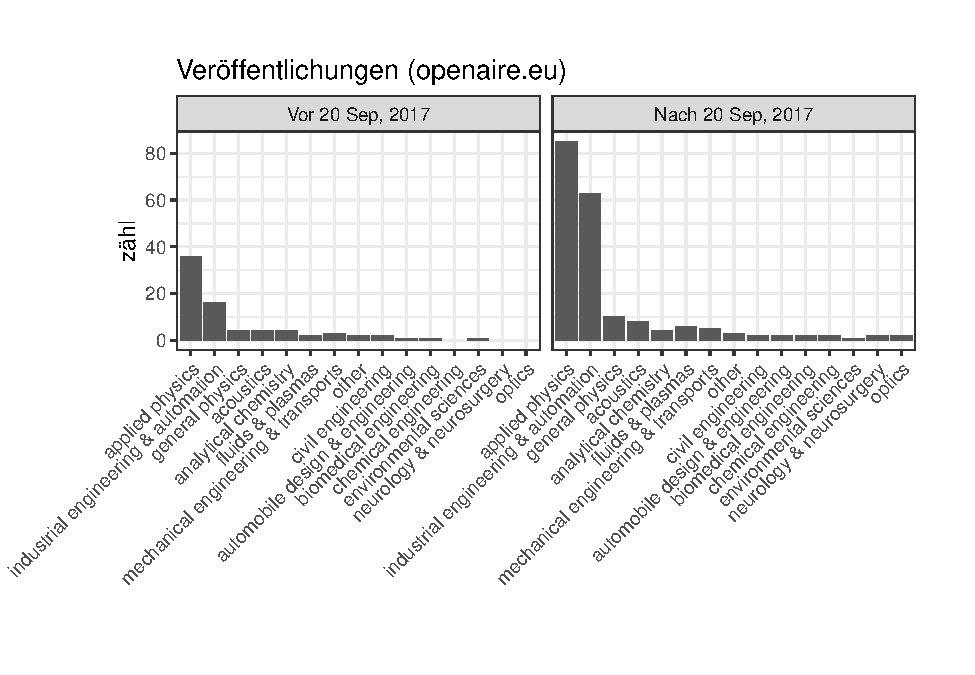
\includegraphics{Linearmotor_schobben_2022_files/figure-latex/plot-1.pdf}
\caption{\label{fig:plot}Veröffentlichungen nach (Teil-)Disziplinen kategorisiert und in zwei Gruppen aufgeteilt: Vor 20 Sep, 2017 und Nach 20 Sep, 2017.}
\end{figure}

Anwendungen in Medizin und Naturwissenschaften legen nahe, dass zukünftige Entwicklungen von Linearmotoren eine weitere Optimierung der Präzision (im Mikro- bis Nanometerbereich) sowie eine weitere Reduzierung von Größe und Gewicht dieser Geräte umfassen werden. Eine genauere Untersuchung der von der OpenAire-Plattform gewonnenen Daten (Abb. \ref{fig:plot}) zeigt, dass weitere Verbesserungen durch die Aufnahme von Störeffekten wie Reibung, Drehmomenten und anderen parasitären Kräften erzielt werden können. Diese aktive Forschungsdisziplin der Linearmotor-Präzisionsoptimierung lässt sich grob in drei Ansätze unterteilen. Das erste Lösungspaket umfasst die Untersuchung neuer Rohstoffe, wie zum Beispiel Hybridmaterialien für Eisenkern-Linearmotoren \citep{liu2021} und Hochtemperatur-Supraleitermagnete für einen energieeffizienteren Stromverbrauch \citep{zhang2016, palka2021}. Das Erfordernis von Seltenerdelementen in diesen Lösungen schränkt die vollständige Implementierung angesichts der Knappheit dieser Ressourcen ein \citep{deboer2013}. Motoren in molekularer Größe, die aus Kohlenstoffnanoröhren bestehen, die durch thermische Gradienten angetrieben werden, und Supraleiter auf Graphenbasis könnten zukünftige Wege zur Größenreduzierung und Energieeffizienz sein, aber diese Materialien sind noch weitgehend experimentell \citep{zambrano2009, cao2018}. Eine zweite Reihe von Lösungen konzentriert sich auf die Verbesserung der Designparameter des Geräts \citep{kuang2017, kramer2021}, während ein dritter Ansatz darauf abzielt, Algorithmen zu verbessern, die Linearmotoren führen, wodurch die Bahnverfolgung verbessert und die Auswirkungen anomaler Kräfte auf die Präzision verringert werden \citep{nguyen2016, mo2017, yunbo2018, chen2020, yao2021}.

\hypertarget{optim}{%
\section{Optimierungspotenziale}\label{optim}}

Das Gewicht der Eisenkernläufer führt aufgrund der erhöhten Trägheit des Systems zu höheren Energiekosten. Im Gegensatz dazu wurden eisenlose Linearmotoren entwickelt, um diese höhere Trägheitsbelastung zu überwinden, indem leichtere Materialien in der Läufer verwendet werden. Bei letzterer Konstruktion sind die Spulen der Läufer in Epoxidharz gegossen. Dies hat einige offensichtliche Vorteile in Bezug auf das Gewicht des Läufer, was zu einer höheren Beschleunigung/Verzögerung von Bewegungen führt. Dennoch haben eisenlose Linearmotoren einige Einschränkungen im Vergleich zur eisenbehafteten Variante, was hauptsächlich zu höheren Nennkräften für ähnlich große eisenlose Varianten führt. Um ähnliche Spezifikationen zu erreichen, müssen einige Einschränkungen des eisenlosen Linearmotors überwunden werden. Diese Einschränkungen lassen sich grob in drei Gruppen einteilen:

\textbf{Materialien} Die Epoxidharz-Läufer von eisenlosen Linearmotoren haben eine geringere Wärmeleitfähigkeit und Struktursteifigkeit als die Variante mit Eisenkern. Dies kann überwunden werden durch:

\begin{itemize}
\tightlist
\item
  Entwicklung besser wärmeleitfähiger Epoxidharze. Dies kann möglicher- weise durch die Verwendung von Nanopartikeleinschlüssen erreicht werden, die in das Epoxidharz eingebettet sind \citep{fu2010}.
\item
  Verbesserung der strukturellen Steifheit des Epoxidharzes. Kunststoffe mit einer hohen strukturellen Steifigkeit sind ein Forschungsschwerpunkt in prothetischen Studien \citep{agha2016}. Diese Fortschritte in der Prothetik könnten möglicherweise in eisenlose Läufer-Designs implementiert werden.
\item
  Verringerung des Gewichts der Spule durch Verwendung von (Hochtem- peratur-)supraleitenden Spulen mit geringerem Energieverbrauch \citep{palka2021}. Noch spekulativer ist die Umsetzung von noch weitgehend theoretischen Supraleitern wie „Magic-Winkel-Graphen`` \citep{cao2018}.
\end{itemize}

\textbf{Designoptimierung} Das Y-Träger-Design ist ein Beispiel für eine geometrische Konfiguration, die den Wirkungsgrad von eisenlosen Linearmotoren verbessert. Aufbauend auf diesen Fortschritten bei der Gestaltung der Streitkräfte kann man:

\begin{itemize}
\tightlist
\item
  weitere Verbesserung der Motorgeometrie und anderer Konstruktions- parameter durch topologische und magnetische Flussmodelle \citep[z. B.][]{duan2011}.
\item
  Präzisionsfertigungsverfahren (z. B. Laser-Metallschneiden) anwenden, um Konstruktionsverbesserungen mit minimalen Abweichungen tatsächlich zu implementieren. Die Minimierung von Produktionsfehlern wird die Effizienz dieser Systeme in realen Anwendungen erhöhen.
\end{itemize}

\textbf{Adaptive Algorithmen} Berechnungsroutinen für die Bewegungsverfolgung und korrigierendes Feedback werden dazu beitragen, die Wechselwirkung des magnetischen Flusses und andere parasitäre Kräfte zu überwinden, die die Leistung der Maschine negativ beeinflussen \citep{nguyen2016}. Solche Algorithmen können profitieren von:

\begin{itemize}
\tightlist
\item
  erhöhte Rechenleistung, die der Bewegungsgeschwindigkeit im mechan- ischen System entspricht. Dies kommt der Gesamtleistung zugute.
\item
  Implementieren von ``self-supervised machine learning'' Algorithmen, die iterativ die beste Routine für bestimmte Bewegungen innerhalb eines bestimmten Systems lernen können.
\end{itemize}

Verbesserungen in all diesen Kategorien können die Leistung des Systems verbessern, ohne dass größere und schwerere Läufer erforderlich sind. Umgekehrt ergeben sich dadurch auch Möglichkeiten, die Größe und das Gewicht von Linearmotoren weiter zu reduzieren. Dies wäre vorteilhaft für Hochpräzisionsanwendungen wie biomedizinische Geräte, chirurgische Werkzeuge und High-End-Optiken, die eine räumliche Präzision im Nano- bis Mikrobereich mit einer sehr konsistenten Geschwindigkeitssteuerung der Bewegung erfordern.

\hypertarget{consortium}{%
\section{Consortium}\label{consortium}}

Basierend auf den Beobachtungen in Abschnitt \ref{optim} scheint ein hohes Potenzial zur Verbesserung der Präzision eisenloser Linearmotoren zu bestehen. Diese spezifischen Geräte haben zahlreiche Hochpräzisionsanwendungen. Daher habe ich das Ziel des Konsortiums um einen bestimmten realen Anwendungsfall herum formuliert. In diesem Konsortium sehe ich die Optimierung des eisenlosen Linearmotordesigns als ein potenziell sehr lohnendes Unterfangen zur Verbesserung der Linearmotorleistung in Exoskeletten (für neuromuskuläre Erkrankungen und Rehabilitation) und Prothetik (intern und extern). Die vorgeschlagenen Lösungen könnten die Präzision mechanischer Bewegungen verbessern, um das menschliche Motorsystem besser nachzuahmen, zu langlebigeren und leichteren Geräten führen, die dem Komfort des Benutzers zugute kommen, und die Batterielebensdauer verlängern. Diese Merkmale wurden als Engpässe bei der Entwicklung von Exoskeletten und Prothesen identifiziert \citep{pasquina2015}. Ich habe die Rollen der Konsortiumsmitglieder wie folgt aufgeteilt: „Materialentwicklung``, „Designoptimierung`` und „Test und Produktion``. Für jede dieser Rollen habe ich eine Reihe von Forschungsinstituten und Unternehmen aufgelistet, die die oben genannten Spezifikationen für die Optimierung von Linearmotoren umsetzen werden.

\textbf{Materialentwicklung} Die Entwicklung von Materialien mit größerer Wärmeleitfähigkeit und struktureller Steifigkeit ist ein entscheidender Aspekt, der das Linearmotor-Design voranbringen könnte, indem die Präzision der Bewegungen und die Haltbarkeit des Läufer erhöht werden.

\begin{itemize}
\tightlist
\item
  \href{https://www.ipfdd.de/de/forschung/institut-fur-makromolekulare-chemie/funktionale-nanokomposite-und-blends/forschungsfelder/kohlenstoffhaltige-verbundwerkstoffe\%20-Nanostrukturen/}{Leibniz-Institut für Polymerforschung}, Dresden: Dieses Institut verfügt über eine Forschungsgruppe, die sich speziell mit der Erforschung des Einflusses von Kohlenstoff-Nanostruktureinschlüssen in Polymere auf thermische Eigenschaften befasst. Dieses Know-how wäre geeignet, Epoxidharze für eisenlose Läufer mit besseren Wärmeleiteigenschaften zu entwickeln.
\end{itemize}

\textbf{Designoptimierung} Das vorgeschlagene Konsortium wird hochmoderne künstliche neuronale Netze kombinieren, um die Designparameter zu optimieren, bevor die eigentliche Produktion beginnt. Künstliche neuronale Netze haben sich als besonders nützlich für die Modellierung nichtlinearer Systeme erwiesen und wurden erfolgreich bei der Topologieoptimierung und Designproblemen von Wärmeleitungssystemen eingesetzt \citep{zhang2021}.

\begin{itemize}
\item
  \href{https://www.iais.fraunhofer.de/}{Fraunhofer-Institut für Intelligente Analyse- und Informationssysteme}, Dresden: Hat eine lange Tradition in der Erforschung intelligenter digitaler Lösungen und der anschließenden Anwendung dieses Wissens auf reale Probleme. Darüber hinaus verfügt das Institut über ein umfangreiches Netzwerk, das Bildungseinrichtungen, Start-ups und Kooperationen enthält, die das Konsortium ergänzen könnten.
\item
  \href{https://www.celus.io/}{CELUS GmbH}, München: Ist ein Künstliche Intelligenz-gestütztes Start-up, das sich auf Elektronik-Engineering-Prozesse konzentriert, darunter: intelligente Lösungen für die Materialauswahl und ``digital twins'' für elektronischer Komponenten. Diese Erfahrung könnte helfen, die Designphase zu erleichtern, aber auch adaptive Rückkopplungsalgorithmen zu konstruieren, die helfen, Bewegungen zu regulieren und unerwünschte Störkräfte (z. B. Magnetflusswechselwirkung und parasitäre Kräfte) zu kompensieren.
\end{itemize}

\textbf{Test und Produktion} Es ist wichtig, über eine Produktionslinie zu verfügen, die dieselbe Genauigkeit wie die in der Designphase verwendeten Parameter liefern kann. Voraussetzung für eine solche Genauigkeit sind eine präzise Fertigung und kritische Qualitätsprüfungen entlang der Produktionslinie. Dies ermöglicht eine reale Erprobung der Geräte in Versuchsaufbauten und ermöglicht einen Vergleich mit dem Modelloutput der Designphase. Darüber hinaus sind Testversuche erforderlich, um die Zufriedenheit der Anwender mit den neu entwickelten Geräten zu testen.

\begin{itemize}
\item
  \href{https://www.faulhaber.com/en/markets/medical/exoskeletons-prosthetics/}{Faulhaber Gruppe}, Schönaich: Ist ein Hersteller von Hightech-Miniatur- und Mikromotoren, darunter Linearmotoren, und sie aktiv Forschungslösungen für den Prothetik- und Exoskelettmarkt. Die jahrzehntelange Erfahrung in der mikroelektronischen Produktion und das Maß an Genauigkeit in ihren Produktionslinien werden die in der Designphase festgelegten Designziele verwirklichen.
\item
  \href{https://www.ottobock.com/de-de/startseite}{Ottobock SE \& Co.~KGaA}, Duderstadt: Diese Firma ist am Ende der Produktionskette für Prothetik- und Exoskelettprodukte angesiedelt. Dieses Unternehmen führt regelmäßig klinische Tests seiner Produkte durch, um die Leistung und Benutzerzufriedenheit zu quantifizieren. Die Ergebnisse dieser Trails können wiederum wichtige Informationen in das Designface einfließen lassen und schließen so den Kreis dieses Forschungs- und Entwicklungsprozesses.
\end{itemize}

\hypertarget{zeitplan}{%
\section{Zeitplan}\label{zeitplan}}

Das Arbeitspaket ``Materialentwicklung'' wird mit Beginn des Projekts beginnen und Ergebnisse in Form von Publikationen und schließlich eines Epoxidharzes liefern, das in den anderen beiden Paketen verwendet werden kann. Arbeitspaket ``Designoptimierung'' beginnt idealerweise, wenn Arbeitspaket 1 ein neues Epoxidharzes liefert, für das die Materialeigenschaften im mathematischen Modelldesign verwendet werden sollen. Arbeitspaket ``Test und Produktion'' erfordert Materialien aus Arbeitspaket 1 und ein fertiges Gerätedesign als Ergebnis von Arbeitspaket 2. Daher beginnt Arbeitspaket 3 als letzte Phase dieses Forschungsplans.

Folgende ``Milestones'' wurden formuliert:

M1. Entwicklung eines neuartigen Epoxidharzes mit hervorragenden Wärmeleiteigenschaften.\\
M2. Entwicklung einer neuartigen Topologie, die das Kraftgewicht reduziert und gleichzeitig die strukturelle Steifigkeit beibehält.\\
M3. Verbessertes Prothesen- und/oder Exoskelettdesign, das den Bedürfnissen der Benutzer entspricht.

\begin{figure}
\centering
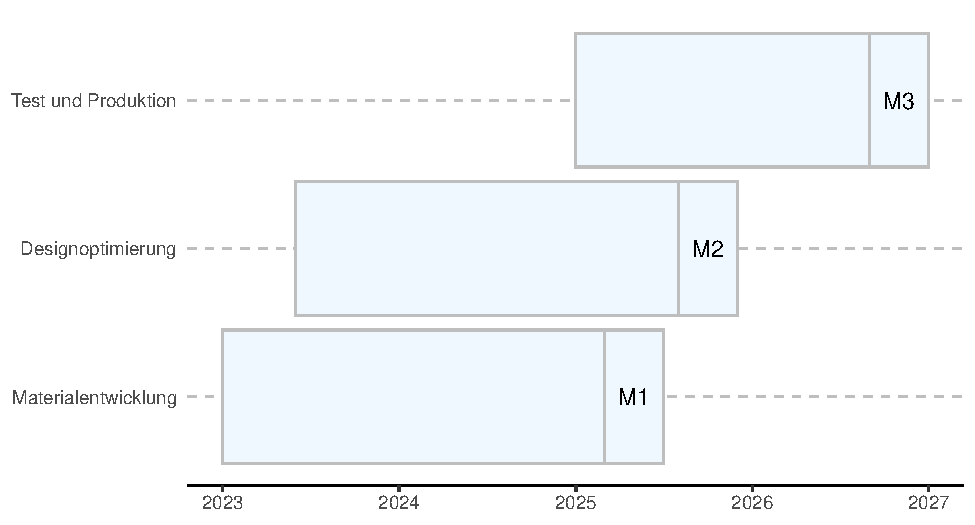
\includegraphics{Linearmotor_schobben_2022_files/figure-latex/gantt-1.pdf}
\caption{\label{fig:gantt}Gantt chart für Case Study ``Linearmotor''}
\end{figure}

  \bibliography{book.bib,packages.bib,linearmotors.bib}

\end{document}
